\documentclass[12pt,a4paper]{article}
\usepackage[utf8]{inputenc}
\usepackage[spanish]{babel}
\usepackage{amsmath}
\usepackage{amsfonts}
\usepackage{amssymb}
\usepackage{graphicx}
\usepackage[T1]{fontenc}
\usepackage{imakeidx}
\usepackage[left=3cm,right=3cm,top=2.5cm,bottom=2.5cm]{geometry} %margen
% \setcounter{page}{5}
\title{Desarollo de una Aplicación que Proporcione Portafolios de Inversion  por Medio  
	del Modelo Fama-French y Cadenas de  Markov}
\linespread{2}
\begin{document}
	\begin{center}
	\textbf{UNIVERSIDAD MARISTA}
	\begin{figure}[htb]
	\centering
	
\includegraphics[scale=1.1]{logo_marista_trabajo_titulacion.jpg}
	\end{figure}\\
	RECONOCIMIENTO DE  VALIDEZ OFICIAL  DE ESTUDIOS\\
	$No. 992135$ DE FECHA 25-II-99, OTORGADO \\
	POR LA SECRETARÍA DE EDUCACIÓN PÚBLICA \\
	\textbf{Desarollo de una Aplicación que Proporcione Portafolios de Inversion  por Medio  
	del Modelo Fama-French y Cadenas de  Markov}\\
	\textbf{Tesís}\\
	QUE PARA OBTENER EL TITULO DE : \textbf{LICENCIADO EN ACTUARÍA}\\
	P R E S E N T A\\
	Arredondo Pérez Leonardo\\
	CIUDAD DE MEXICO 2022\\
	\end{center}
\newpage
\tableofcontents
\newpage
\listoffigures
\addcontentsline{toc}{chapter}{Índice de figuras}
\newpage
\listoftables
\addcontentsline{toc}{chapter}{Índice de tablas}
\newpage
	\section {Introducción}
	\hfill\break
	En esta investigación, desarollaremos una aplicación web, la cual  ortogara una serie de portafolios de inversión a tiempo discreto. Estos portafolios se haran dependiendo de las empresas seleccionadas por el usuario, el  monto a invertir, la temporalidad de reinversión y el nivel de riesgo que este dispuesto a asumir.\\
	\hfill\break
	Para poder tener una relación adecuada entre nuestro riesgo y rendimientos,  tenemos que seleccionar un modelo finaicero, el cual debe reflejar el comportamiento del mercado, es por eso que se selecciono el modelo Fama-French, ya que se ah demostrado que los rendimientos de los mercados se pueden obtener con regresiones lineales.\\
	\hfill\break
	Sin embargo, para poder cumplir nuestro objetivo, no es suficiente el uso del modelo Fama-French, debido a que solo nos otorga un perido de inversión, por lo que  utilizaremos cadenas de Markov y simulaciones, para poder ofrecer portafolios con una mayor perodicidad. \\
	\hfill\break
	En el capitulo I abordaremos el tema de aplicaciones web, vermos sus tipos, usos y daremos la  estrucutara nuestra aplicación.\\
	\hfill\break
	En el capitulo II presentaremos al modelo Fama and French, este modelo sera nuestra base para poder cálcular las pondereaciones de nuestros portafolios.\\
	\hfill\break
	En el capitulo III hablaremos sobre las cadenas de MarKov, con el apoyo de este proceso estocastico, calcularemos las probabilidades de transicción, en el cambio de estados para los rendimientos.\\
	
	\newpage
	\section{Problematica}
	\hfill\break
	A lo largo de la historia las personas han tenido la necesidad de realizar intercambios de bienes y servicios, cuando
	las necesidades de estas transacciones fueron evolucionando  las personas tuvieron que crear  un sistema financiero, daondele seguridad  y regulación a estos intercambios,se define un sistema financiero de acuerdo con  (BANXICO, s.f.) como:\\
	\hfill\break
	$"$El conjunto de instituciones, mercados e instrumentos en el que se organiza la actividad financiera, para movilizar el ahorro a sus usos más eficientes.$"$\\
	\break
	En la figura 1 exponemos, la estructura del sistema financiero mexicano.\\
	Como podemos observar, los princaples entes de este son: El Banco de México y la Secretaria de Hacienda y Credito Publico (SCHP). EL Banco de México, cumple con la fución de agente finciero por parte del gobiernos en los mercados financieros.\\
	\begin{figure}
		\centering
		\caption{Estructura del Sitema Financiero Mexicano}{{\footnotesize Fuente: Elaboración propia-Igleses, s.f.}}
		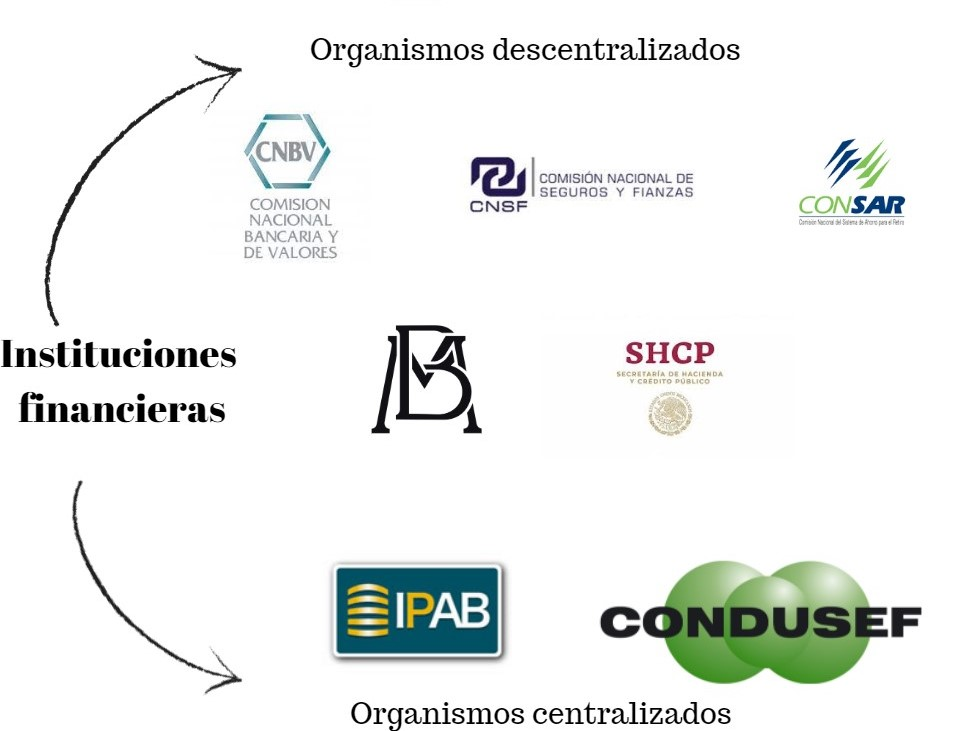
\includegraphics[scale=0.4]{estructurasfm.jpg}
	\end{figure}
	\newpage
	\hfill\break
	En  nuestro sistema financiero, tenemos tres  tipos de mercados fincieros, un mercado finanicero, de acuerdo con (Garcia,2018 ) es:\\
    \hfill\break
	$"$ Un espacio físico o sistema virtual en el cual convergen compradores y vendedores de instrumentos financieros para su intercambio $"$\\
	\hfill\break
    En México contamos con el mercado de deuda, en el cual se negocian titulos de deuda \\
    El mercado de divisas, en este se pone el precio de una divisa respecto a otra,  por medio de  la compra y venta de estas.\\
    
	Por ultimo, contamos con el mercado de acciones o de capitales, el Instituto de la Bolsa Internacional de Valores (BIVA), este se define como:\\
	\hfill\break
	$"$El mercado de valores es el espacio en el que las empresas o gobiernos colocan instrumentos de deuda o capital (como las acciones) con el fin de financiarse de forma  segura, rentable y a cualquier plazo.$"$\\
	\hfill\break
	Como menciona BIVA, una de las formas en las que las empresas pueden adquirir, un finaniciamiento, es ofertando instrumentos finaniceros, denominadas acciones.\\
	La importancia que tiene el sistema finciaero es poder realizar la compra y venta de los instrumentos financieros, de una manera transparente  y verificar que se cumplan con lo estipulado en las transacciones finaiceras.\\
	
    Para nuestra investigación, nos enfocaremos en el mercado de capitales.\\
    Para poder hacer una inversión de forma racional, lo más conveniente es la diversificación, esta nos ayuda  a recompenzar aquellas posibles perdidadas que podamos  llegar a tener con las ganancias.\\
    
    \hfill\break
    La pregunta a resolver, al momento de generar un portafolio, es : ¿Qué poderanción debe terner cada una de nuestas accciones, de tal manera que se minimice nuestro riesgo y se maximice nuestras ganancias?, para esto nos podemos apoyar de los diferentes modelos desarollados, como el Modelo de Markovitz, tambien conocido como media-varianza, el cual nos proporciona un portafolio optimo con las siguientes formulas para calcular estos porcentajes.\\
    En la figura 2 mostramos la frontera eficeinte y la de mínima varianza.
    \hfill\break
    \begin{figure}
		\centering
		\caption{Fronteras eficientes y de mínima varianza}{{\footnotesize Fuente: Elaboración propia}}
		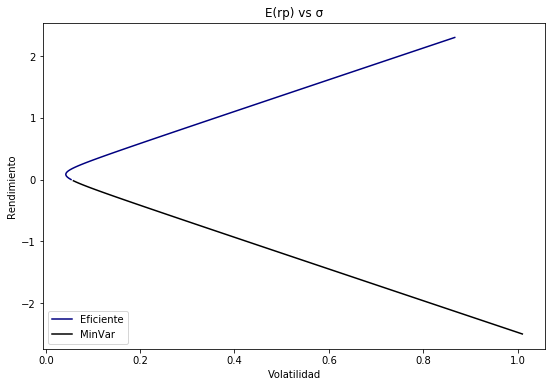
\includegraphics[scale=0.6]{markovitz.png}
	\end{figure}
	\hfill\break
	Asi mismo, se cuenta con el modelo Capital Asset Pricing Model (CAPM),el cual nos proporciona los rendimientos esperados, para poder utilizarlo, debemos de ralizar una regresión lineal, del comportamiento del mercado respecto a nuestra empresa, esta regresión lineal, nos dara la una pendiente y una ordenada al origen, las cuales representaran nuestro rendimiento y rendimiento respectivamente.Con la siguiente formula podemos estimar el rendimiento de nuestro activo.\\
	Ecuación de la regresión lineal\\
	$$y=\alpha x+\beta$$
	Ecuación para cálcular el rendimiento de acuerdo con el CAPM\\
	$$R_{a} = R_{rf} + \beta \alpha* (R_{m} - R{rf})$$\\
	En la siguiente figura, se expone un ejemplo de la aplicación de este modelo.\\
	\hfill\break
	\begin{figure}
		\centering
		\caption{Google respecto al índice IPC}{{\footnotesize Fuente: Elaboración propia}}
		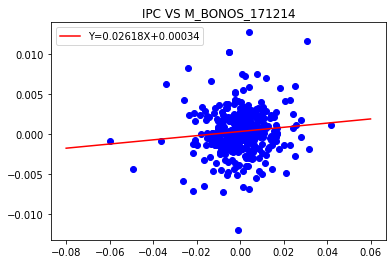
\includegraphics[scale=0.6]{ejmplo_CAPM.png}
	\end{figure}
	\hfill\break
    Por utlimo, tenemos el  modelo fama french FAMA-FRENCH, cuyo objetivo principal es estimar los rendimientos de un activo considerando los siguientes factores
     \textbf{Factor 1:}Riesgo de mercado\\
    \textbf{Factor 2 }: El rendimiento de las empresas de peque˜na capitalizaci´on en relaci´on a las empresas de gran capitalización. Por sus siglas en ingles Small Minus Big (SMB)\\
    \textbf{Factor 3 } El rendimiento superior de las empresas de mayor capitalización, por sus siglas en íngles (High Minus Low)\\
    Una vez obtenido los valores de estos factors, se obtendra el rendimiento de nuestro activo
    con la siguiente ecuación:\\
    $$r = r_{f} + \beta_{1}(r_{m} − r_{f} ) + \beta_{2}(SBM) + \beta_{3}(HML)$$
    \newpage
	\section{Justificación}
	\hfill\break
	%%Sobre el modelo
	Como podemos observar, existen, diversos metodos para poder calcular, las ponderaciones de un portafolio, sin embargo, existen estudios que demuestras que no todos son utiles al momento de llevarlo a la vida practica, añadiendo que estos modelos solo nos otorgan   los porcentajes de nuestra cartera, para un solo periodo.\\
	Como mencionan   Chen, J. y Kawaguchi, Y(2018)\\
	\hfill\break
	$"$Aunque el modelo de media-varianza, CAPM y el modelo multifactorial son lógicamente simples y útiles en la práctica, son modelos lineales estáticos de un solo período, que difícilmente pueden ajustarse al mundo real (p1)$"$\\
	\hfill\break
	
	Tomando en cuenta lo anterior, para la selección de los porcentajes de nuestro portafolio, debemos de seleccionar un modelo que tenga evidencia de ser util en la practica. Para poder ofrecer portafolios a más de un periodo, tenemos que estar fudamentados con procesos estocasticos, que nos midan la probabilidad de cambios de régimen de los rendimientos.\\

	Esta aplicación es creada para que las personas que no esten tan familiarizadas con los temas de inversión,  puedan obtener un rendimiento, que lo puedan hacer de manera senciila y facil de manipular.\\
	
	\section{Formulación del problema}	
	¿Con qué nivel de confianza podemos asegurar que los portafolios generados en nuestra aplicación, nos den un retorno de la inversión mayor al
	 $100\%$?
	\section{Objetivos}
	\subsection{General}
			Desarollar una apliación, que proporcione portafolios de inversión, con el uso del modelo de Fama-French y cadenas de Markov, que nos otorguen un retorno sobre la  inversion mayor a $100\%$.
	\subsection{Especificos}
			\begin{enumerate}
			    \item Obtener por medio de un formulario, el monto a invertir, el nivel de riesgo a asumir, la periodicidad para la reinversión y las empresas en las cuales vamos a invertir.
			    \item Calcular el portafolios que reflejen el comportamiento del mercado de acuerdo al modelo Fama and French.
			    \item Cálcular las matricez de transicción, de cambio de regimen en los rendimientos de las empresas, por medio de las cadenas de Markov.
			    \item Modelar los precios de las empresas con ecuaciones diferenciales estocasticas.
			    \item Proporcionar los  portafolios a invertir.		
			 \end{enumerate}		
	\section{Marco Teórico}
	\subsection{Capítulo 1: Aplicaciónes Web}
	\hfill\break
	\subsection{Capítulo 2: Modelo Fama and French}
	\hfill\break
	\subsection{Capitulo 3: Cadenas de Markov}	
	\hfill\break
	\section{Metodologia}
	\hfill\break
	\section{Resultados}
	\hfill\break
	\section{Concluciones}
	\hfill\break
	\section{Bibliografía}
	\hfill\break
	\begin{enumerate}
	    \item Chen, J., y Kawaguchi, Y. (2018). Multi-factor asset-pricing models under markov regime switches: Evidence from the	chinese stock market. International Journal of Financial Studies, 6(2), 54.
	    \item  La guía definitiva del modelo de tres factores Fama-French. (2019, 2 octubre). Affde. Recuperado  09 de septimebre de 2022, de https://www.affde.com/es/fama-french-three-factor-model-guide.html
	    \item Banxico Informa,s.f Mercados financieros. Recuperado 9 de septiembre de 2022, de http://educa.banxico.org.mx/$banco\_mexico\_banca\_central$/sist-finc-mercados-financiero.html
	\end{enumerate}				
\end{document}